\hypertarget{P116}{}
\begin{solution}{normal} % 116
Determine the magnetic field at a distance $x$ along the axis of a loop of current. The loop has radius $R$ and has a current $I$ running through it.
\end{solution}

\hypertarget{P117}{}
\begin{solution}{normal} % 117
Determine the magnetic field due to an infinite sheet of current. The current density ($\text{A}/\text{m}$) is everywhere and equal to $\alpha$.
\end{solution}

\hypertarget{P118}{}
\begin{solution}{normal} % 118
Determine the magnetic field at a distance $r$ from an infinitely long straight wire. The current in the wire is $I$.
\end{solution}

\hypertarget{P119}{}
\begin{solution}{normal} % 119
Determine the magnetic field at a distance $r$ from the axis of a cylindrical conductor if the current density over the cross-section of the conductor is uniform and equal to $J$. The radius of the cylinder is $R$.
\end{solution}

\hypertarget{P120}{}
\begin{solution}{normal} % 120
A solenoid is a thin wire that is tightly and evenly wrapped in a cylindrical manner. Consider a long solenoid with $n$ turns per unit length along its axis with a current $I$ passing through it. Such a solenoid is the magnetic analogue of a parallel plate capacitor. Show that: a) the magnetic field inside the solenoid is homogeneous and oriented in the axial direction; b) there is no magnetic field outside the solenoid, and c) the magnetic field inside the solenoid is given by $B=\mu_0nI$.
\end{solution}

\hypertarget{P121}{}
\begin{solution}{normal} % 121
The figure below depicts two different wires each with current $I$ running through it (straight branches run to infinity). In each case, determine the magnetic force at the point marked with a black dot.
\begin{center}
    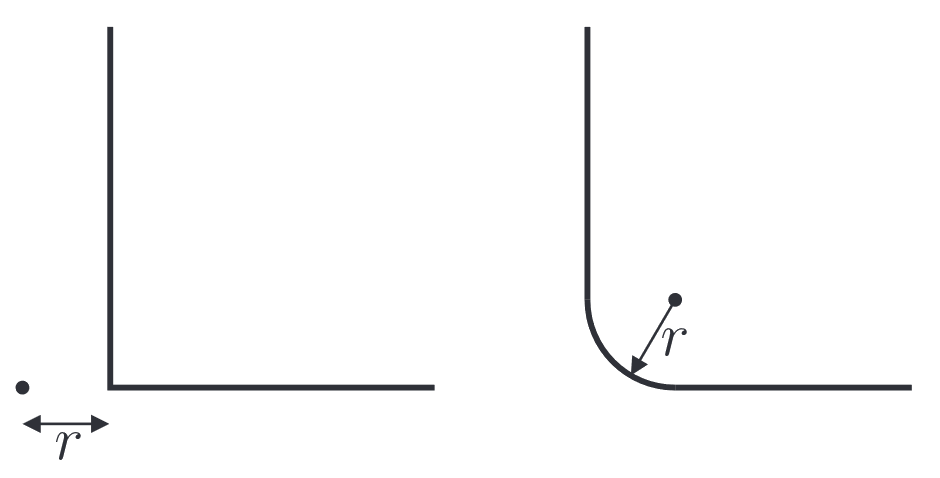
\includegraphics[width=0.5\textwidth]{S4 Figures/S4-121.png}
\end{center}
\end{solution}

\hypertarget{P122}{}
\begin{solution}{normal} % 122
Determine the magnetic field at the end of a long solenoid. A current $I$ runs through the solenoid, which has $n$ turns per unit length.
\end{solution}

\hypertarget{P123}{}
\begin{solution}{normal} % 123
Determine the magnetic field in the cavity formed by the intersection of two straight, infinitely long, cylindrical conductors as shown in the figure below. The current densities in each of the conductors are equal but in opposite directions ($\pm J$), the radius of both conductors is $R$, and the distance between their centers is $d$.
\begin{center}
    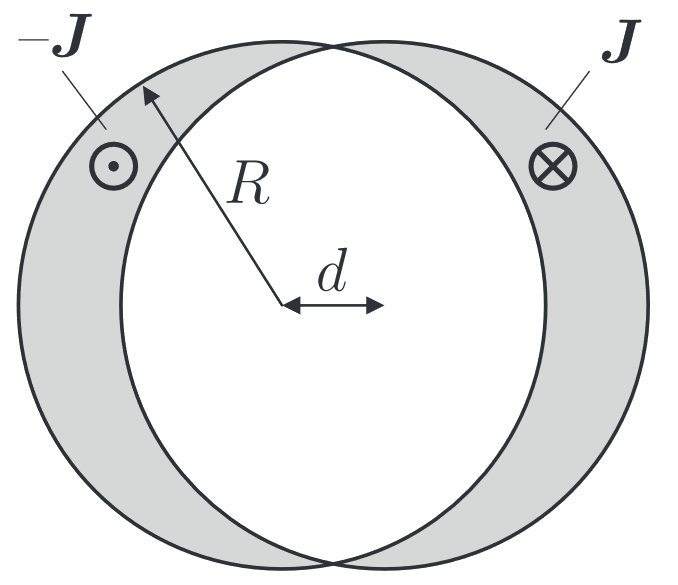
\includegraphics[width=0.35\textwidth]{S4 Figures/S4-123.png}
\end{center}
\end{solution}

\hypertarget{P124}{}
\begin{solution}{normal} % 124
Determine the force per unit length between two infinitely long straight parallel wires if the currents in the wires are $I_1$ and $I_2$ and the distance between the wires is $r$.
\end{solution}

\hypertarget{P125}{}
\begin{solution}{normal} % 125
A charge $Q$ is evenly distributed over a sphere of radius $R$. The sphere rotates at an angular velocity $\omega$ about an axis through its center. Determine the magnetic moment of such a system. \textit{Note:} Divide the surface of the sphere into infinitely thin layers and add the area of a thin spherical segment $\Delta S=2\pi R\Delta h$.
\end{solution}

\hypertarget{P126}{}
\begin{solution}{normal} % 126
A permanent magnet is hung by a thread. Its magnetic moment is $\textbf{\textit{p}}$ (which lies on a horizontal plane) and its moment of inertia from the attachment point of the thread relative to the vertical axis is $I$. Determine the oscillation period of small-amplitude oscillations when a homogeneous horizontal magnetic field $B$ is generated in space.
\end{solution}

\hypertarget{P127}{}
\begin{solution}{normal} % 127
Two permanent magnets (with magnetic moments $\textbf{\textit{p}}_1$ and $\textbf{\textit{p}}_1$) are placed a distance $r$ from each other (where $r$ is much greater than the dimensions of the magnets). Determine the force acting between the magnets.
\end{solution}

\hypertarget{P128}{}
\begin{solution}{normal} % 128
The ratio of the magnetic moment of a particle to its angular momentum is known as the gyromagnetic ratio of that particle. Find the gyromagnetic ratio for the orbital motion of an electron using the Bohr model. \textit{Note:} According to Bohr's theory, the electron orbits the nucleus in a circular orbit where the orbital momentum of the electron is quantized: $mvr=n\hbar$, where $n=1,2,3\dots$.
\end{solution}

\hypertarget{P129}{}
\begin{solution}{normal} % 129
The magnetic moment of an iron atom is given by $p=2.2\mu_B$, where $\mu_B= e\hbar/2m_e\approx9.27\times10^{-24}\;\text{A}\;\text{m}^2$ (also known as the Bohr magneton). The distance between adjacent atoms in the cubic crystal lattice of iron is $d=2.3\;\AA$. What is the maximum magnetic field that can be generated by magnetized iron in the absence of an external magnetic field?
\end{solution}

\hypertarget{P130}{}
\begin{solution}{normal} % 130
Determine the magnetic field inside an infinitely long solenoid if the solenoid is filled with a substance with relative magnetic permeability $\mu$. The ampere-turns per unit length of the solenoid is given by $nI$.
\end{solution}

\hypertarget{P131}{}
\begin{solution}{normal} % 131
A spherical magnet with relative magnetic permeability $\mu$ is placed in a homogeneous magnetic field $\textbf{\textit{B}}_0$. Determine the magnetic field inside the sphere. \textit{Tip:} the magnetic field of a uniformly magnetized sphere outside the sphere is similar to the field produced by a magnetic dipole placed in the center of the sphere.
\end{solution}

\hypertarget{P132}{}
\begin{solution}{normal} % 132
An electromagnet used in a laboratory consists of an iron core (with relative magnetic permeability $\mu$) and a wire wound around it $N$ times, as shown in the diagram below. The width $d$ of the air gap is much smaller than the thickness of the core. If the length of the core is $l$ and the current in the wire is $I$, determine the magnetic field in the air gap of the core.
\begin{center}
    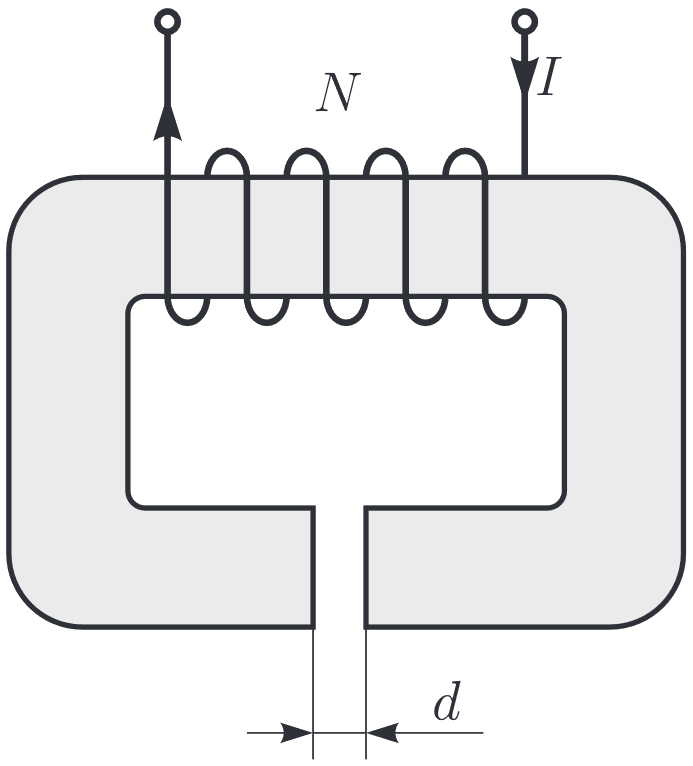
\includegraphics[width=0.6\textwidth]{S4 Figures/S4-132.png}
\end{center}
\end{solution}

\hypertarget{P133}{}
\begin{solution}{normal} % 133
The electromagnet shown below consists of a core (1) and and an anchor (2); the relative permeability of each is $\mu$. A wire is wrapped $N$ times around the core, through which a current $I$ is passed. The cross-sectional area of the core and anchor is $S$ and it has total length $l$. Find the force by which the core holds the anchor. \textit{Note:} A virtual shift method can be used here. However, note that changing the distance between the core and anchor induces an emf in the coil.
\begin{center}
    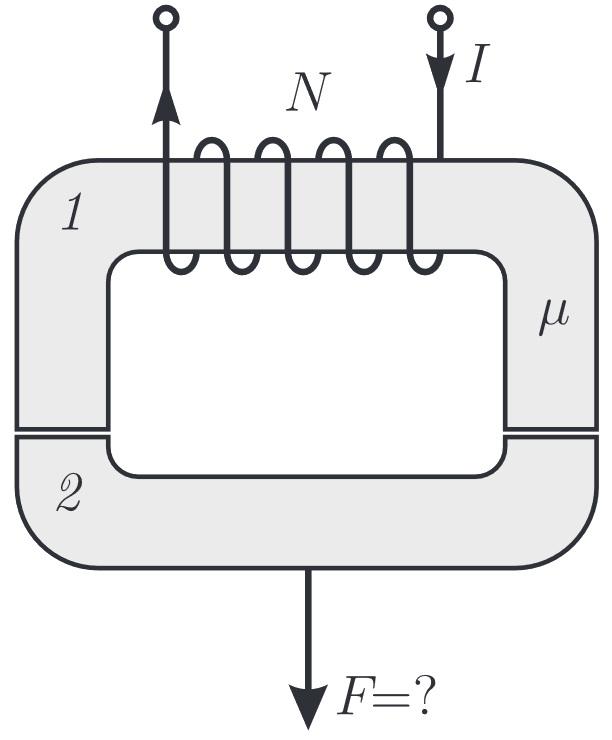
\includegraphics[width=0.6\textwidth]{S4 Figures/S4-133.png}
\end{center}
\end{solution}

\hypertarget{P134}{}
\begin{solution}{normal} % 134
Parallel to and at a distance $h$ above the surface of an infinite planar superconductor is an infinitely long straight wire with current $I$ running though it. Determine the force acting on a unit length of this wire.
\end{solution}